\paragraph{}
O \textit{platooning} é uma coleção de veículos que circulam em conjunto, estritamente espaçados e coordenados entre si em formação, sem violar quaisquer restrições de segurança. Todos os veículos  do pelotão comportam-se da mesma forma que o veículo líder e todas as abordagens de pelotão exigem algum grau de automatização. Esta definição é importante para o desenvolvimento e enquadramento das abordagens já que descreve uma visão genérica sobre o \textit{platooning}.\vspace{5mm} 
Existem também dois aspetos importantes nas abordagens do  \textit{platooning} que são:
\begin{itemize}
\item \textbf{Coordenação de pelotões} – que descreve interações entre pelotões, isto é, pelotões ou veículos, interagem com outro pelotão. Como por exemplo a entrada e saída de veículos de um pelotão
\item \textbf{Controlo de pelotões} – esta abordagem descreve uma visão técnica sobre o pelotão, portanto refere-se à gestão do pelotão. Como por exemplo a gestão do espaçamento entre veículos ou a preparação do pelotão para assumir o controlo de um veículo. 
\end{itemize}
\paragraph{}
As definições de alto nível descritas anteriormente são fundamentais, pois mostra a um investigador  como construir um ambiente de \textit{platooning} sem olhar a pormenores.


\begin{figure}[H]
    \centering
    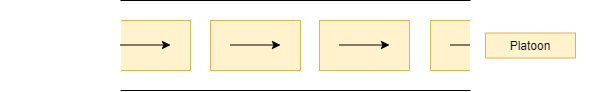
\includegraphics[scale=0.4]{LEI - Article/Images/platooning_trad.png}
    \caption{Platooning "Tradicional"}
    \label{fig:my_label}
\end{figure}